% ============================================================
%  SECTION 11 (was D): When currencies collapse     (Member 4)
%  At merge: 1991 wording and devaluation size aligned with Section 6;
%  India's reserves aligned with Section 7 (RBI, 2026c).
% ============================================================
\section{When currencies collapse: crises in South Asia}\label{sec:crises}

Foreign exchange reserves work like a family's savings for a bad year \seesec{sec:reserves}. But what happens when the savings run out? A country that cannot find enough dollars to pay for its imports and repay its foreign loans can no longer protect its currency. The result is a \keyterm{currency crisis}{A sudden and large fall in the value of a country's currency, usually because the country has run short of foreign exchange.}: a sudden, steep fall in the value of a currency, usually together with shortages and soaring prices. Two of India's neighbours have lived through one recently.

\minihead{Sri Lanka, 2022.} Sri Lanka's troubles built up over several years. Large tax cuts in 2019 reduced the government's income. The COVID-19 pandemic then emptied the tourist hotels that had earned much of the country's foreign currency, while big repayments on foreign loans kept falling due. The central bank held the Sri Lankan rupee at about 200 per dollar and spent its reserves to do so. By the end of March 2022, gross reserves were down to about US\$1.9 billion, and most of that could not easily be spent (Daily Mirror, 2022).

Once the currency was allowed to float in March 2022, it crashed, from about 202 rupees per dollar in February to about 356 by May (Figure~\ref{fig:srilanka}). Fuel, cooking gas and medicines ran short, and people queued for hours outside petrol pumps. In April 2022 the government stopped paying its foreign debts, Sri Lanka's first \keyterm{sovereign default}{When a government fails to make the payments on its debt that it has promised.}. Inflation reached 69.8 per cent in September 2022 (Central Bank of Sri Lanka [CBSL], 2022). In March 2023 the IMF approved a loan of about US\$3 billion (International Monetary Fund [IMF], 2023a), and prices slowly began to settle.

\begin{figure}[!htb]
  \centering
  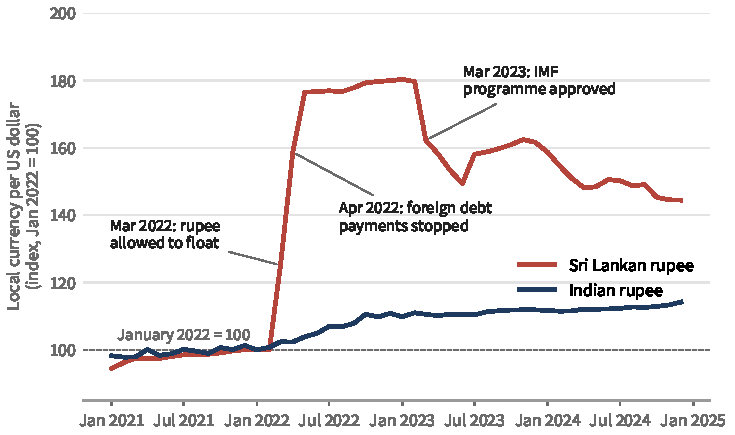
\includegraphics[width=\linewidth]{figures/srilanka_index.pdf}
  \caption{The Sri Lankan and Indian rupees against the US dollar, 2021 to 2024.}
  \label{fig:srilanka}
  {\raggedright\small\sffamily Both lines show how many units of local currency it takes to buy one dollar, scaled so that January 2022 = 100. A rise means the currency has weakened. Once Sri Lanka stopped defending its rupee, it lost value within weeks. The Indian rupee also weakened over 2022, but gradually.\par}
  \figsource{Board of Governors of the Federal Reserve System (2026a, 2026b), series EXINUS and EXSLUS, monthly averages, retrieved from FRED, 1 November 2026. Index calculated by the authors.}
\end{figure}

\minihead{Pakistan, 2022--23.} Pakistan came close to the same edge. High oil prices widened its current account deficit, floods in the summer of 2022 destroyed crops and homes, and talks with the IMF stalled. In early February 2023, the State Bank of Pakistan's reserves fell to about US\$2.9 billion, their lowest level in nine years and barely enough for a few weeks of imports (Business Recorder, 2023a). The government restricted imports and the Pakistani rupee slid, reaching a record low of about 307 per dollar in September 2023 (Xinhua, 2023). Inflation hit 38 per cent in May 2023 (Business Recorder, 2023b). A US\$3 billion \keyterm{IMF programme}{A loan from the International Monetary Fund to a country short of foreign currency, paid in instalments on condition that the country carries out agreed policy changes.}, approved in July 2023, helped Pakistan avoid default (IMF, 2023b).

\minihead{What about India?} Both stories echo India's own crisis of 1991 \seesec{sec:systems}, when reserves covered only about two weeks of imports. India's position today is much stronger. Its reserves stood at about US\$682 billion in May 2026, enough for about 11 months of imports (RBI, 2026c). Under a managed float, the rupee adjusts a little every day, so pressure is released gradually instead of building up behind a fixed rate. And earnings from software services and remittances cover a large part of the gap in goods trade \seesec{sec:bop}.

\begin{table}[!htb]
\centering\small\sffamily
\caption{Three currency crises compared.}\label{tab:crises}
\begin{tabularx}{\linewidth}{@{}>{\raggedright\arraybackslash}p{24mm}>{\raggedright\arraybackslash}X>{\raggedright\arraybackslash}X>{\raggedright\arraybackslash}X@{}}
\toprule
 & \textbf{India, 1991} & \textbf{Sri Lanka, 2022} & \textbf{Pakistan, 2022--23}\\
\midrule
\textbf{Main triggers} & Oil price spike during the Gulf War; fall in remittances; large fiscal and current account deficits & Tax cuts; collapse of tourism during COVID-19; heavy foreign debt repayments; a sudden ban on chemical fertilisers that hurt harvests & High oil prices; large current account deficit; 2022 floods; political uncertainty; stalled IMF talks\\
\addlinespace
\textbf{Reserves at the worst point} & About two weeks of imports & About US\$1.9 billion (March 2022) & About US\$2.9 billion (February 2023)\\
\addlinespace
\textbf{What happened to the currency} & Devalued by about 18--20 per cent in two steps (1--3 July 1991) & Fell from about 202 to about 356 per dollar within three months of floating & Slid to a record low of about 307 per dollar (September 2023)\\
\addlinespace
\textbf{Peak inflation} & 13.7\% (1991--92, wholesale prices) & 69.8\% (September 2022) & 38\% (May 2023)\\
\addlinespace
\textbf{The way out} & IMF loan, gold pledged abroad and wide-ranging economic reforms & Default on foreign debt (April 2022); IMF programme of about US\$3 billion (March 2023); debt restructuring & IMF Stand-By Arrangement of US\$3 billion (July 2023); curbs on imports\\
\bottomrule
\end{tabularx}
\figsource{Business Recorder (2023a, 2023b); CBSL (2022); Daily Mirror (2022); IMF (2023a, 2023b); Xinhua (2023); RBI (n.d.) and Section~\ref{sec:systems} for India, 1991.}
\end{table}

The lesson from all three cases is that currencies rarely collapse because of a single bad event. Low reserves, heavy foreign-currency debt and a large current account deficit are like dry wood. A pandemic, an oil shock or a flood only supplies the spark.

\begin{economistsdisagree}{Is the IMF's medicine too bitter?}
IMF loans come with conditions. Under its 2023 programme, for example, Sri Lanka agreed to raise taxes and to price fuel and electricity so that they cover their costs.

Supporters argue that the conditions fix the problems that caused the crisis in the first place. They also reassure other lenders and investors, who return only when they trust the government's plans. Without reform, they say, the loan would simply be spent and the crisis would return.

Critics reply that raising taxes and cutting spending in the middle of a crisis makes the slump deeper. The burden falls hardest on poor families, who spend most of their income on food and fuel. And conditions drawn up in Washington may not suit local circumstances.

What do you think? Should help in a crisis come with strings attached?
\end{economistsdisagree}
